\documentclass{beamer}

\usepackage[utf8]{inputenc}
\usepackage[T1]{fontenc}
\usepackage{graphicx}
\usepackage{listings}
\usepackage{xcolor}

\useinnertheme{uconn}
\useoutertheme[watermark=corner,logo=stacked]{uconn}
%\useoutertheme[footline=authorinstitute,subsection=true]{miniframes}
%\useoutertheme{sidebar}
\usecolortheme{default}
\usefonttheme{default}

\title[An introduction to Python]{The introduction to Python}
\subtitle{Parallel session of UCSAS 2020}
\author[Jin]{Jun Jin, PhD student}
\institute[UConn]{Department of Statistics\\ University of Connecticut}
\date{\today}

\setlength{\parskip}{.5em}

\lstdefinestyle{Python}{
    language        = Python,
    basicstyle      = \tiny,
    keywordstyle    = \color{blue},
    keywordstyle    = [2] \color{teal}, % just to check that it works
    stringstyle     = \color{green},
    commentstyle    = \color{red}\ttfamily
}


\begin{document}

\lstset{
    frame       = single,
    numbers     = left,
    showspaces  = false,
    showstringspaces    = false,
}

\begin{frame}
\titlepage
\end{frame}

\section{Installation \& Run}

\begin{frame}[fragile]{Installation}
\uncover<1->
{
	\begin{picture}(0,0)(0,0)
		\put(10,-15)
		{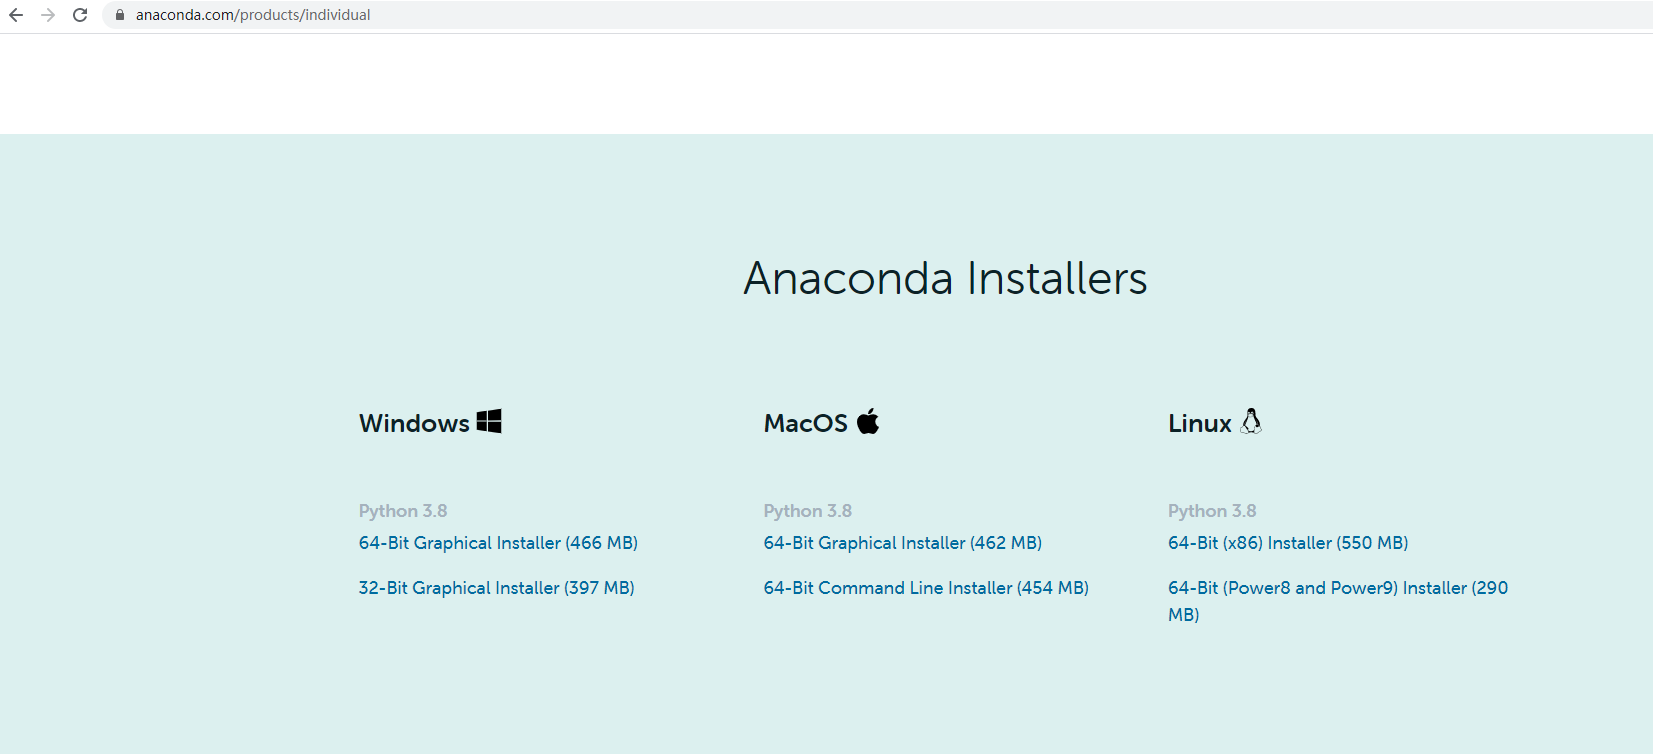
\includegraphics[width=7cm]{images/fig1.png}}
	\end{picture}
}

\uncover<2->
{
	\begin{picture}(0,0)(0,0)
		\put(50,-70)
		{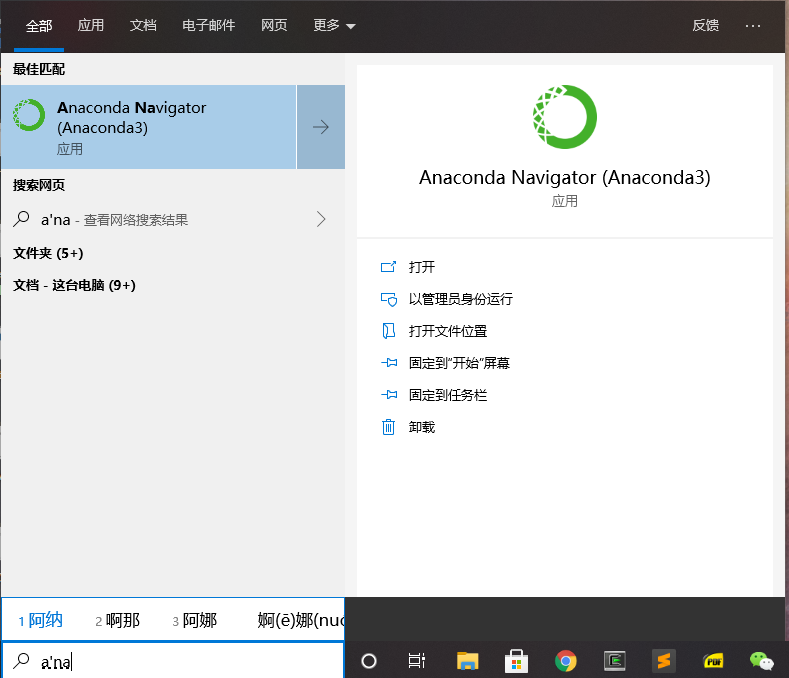
\includegraphics[width=7cm]{images/fig2.png}}
	\end{picture}
}

\uncover<3->
{
	\begin{picture}(0,0)(0,0)
		\put(90,-120)
		{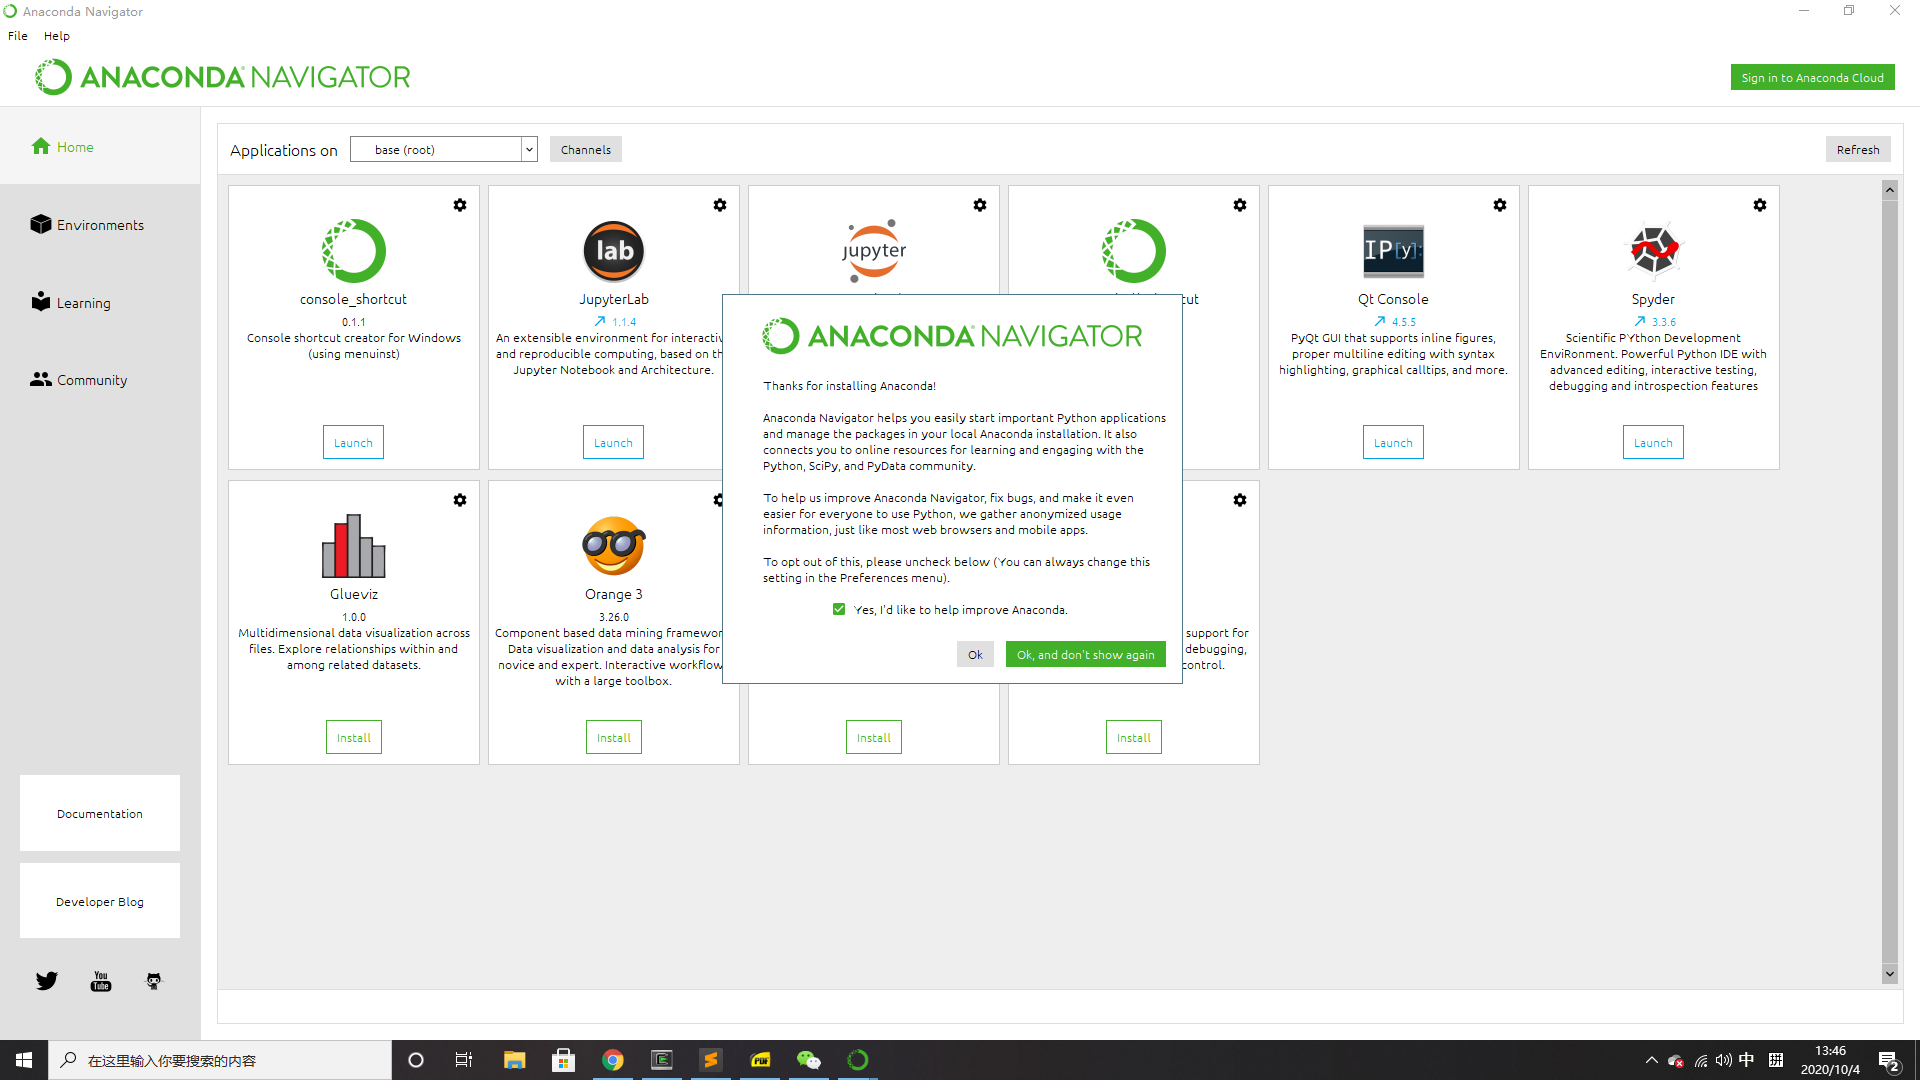
\includegraphics[width=7cm]{images/fig3.png}}
	\end{picture}
}

\end{frame}

\begin{frame}[fragile]{Package management}
\uncover<1->
{
	\begin{picture}(0,0)(0,0)
		\put(10,-80)
		{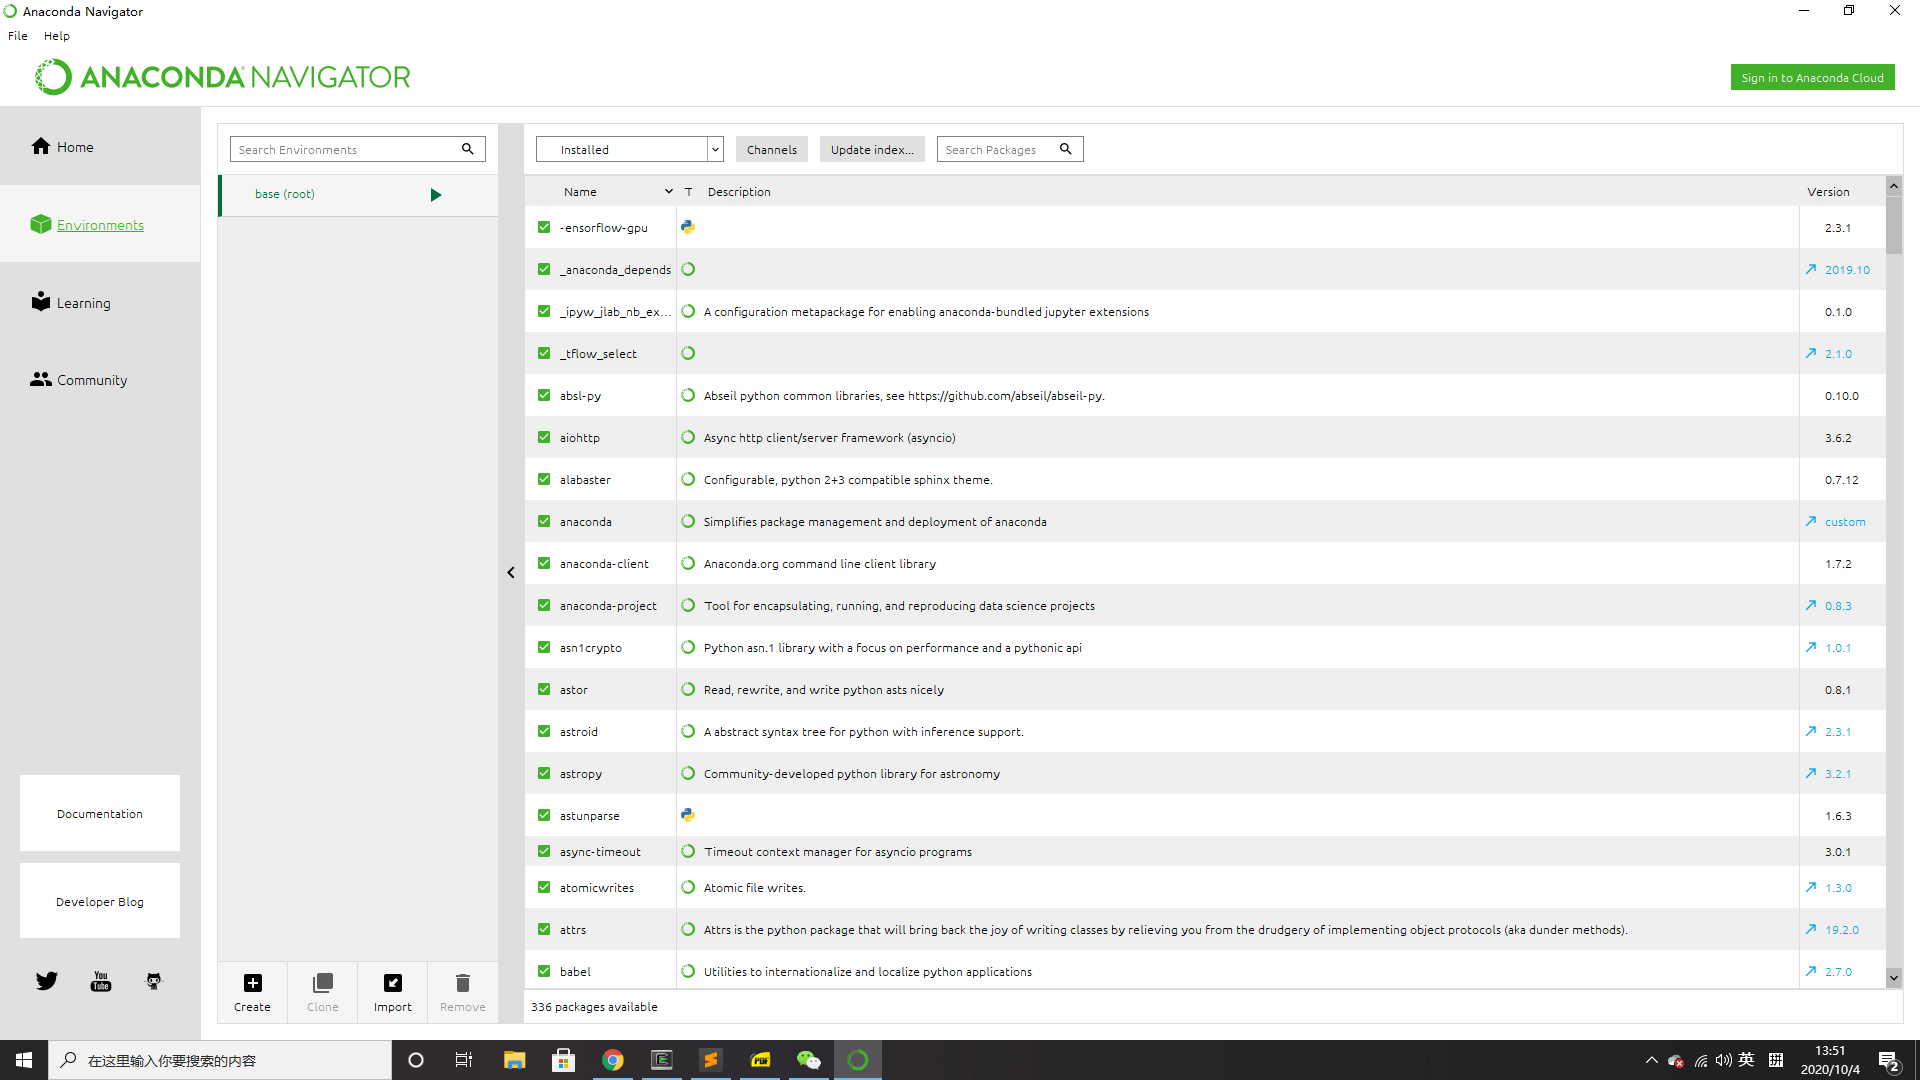
\includegraphics[width=9cm]{images/fig4.png}}
	\end{picture}
}

\uncover<2->
{
	\begin{picture}(0,0)(0,0)
		\put(90,-120)
		{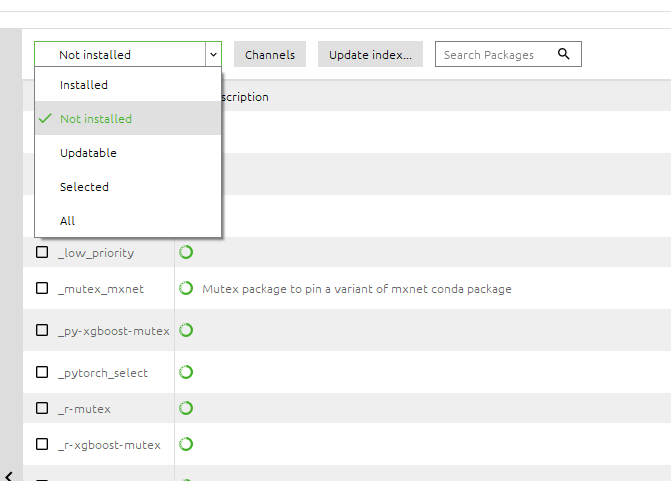
\includegraphics[width=7cm]{images/fig5.png}}
	\end{picture}
}
\end{frame}


\begin{frame}[fragile]{Workspace and launch jupyter}
\uncover<1->
{
	\begin{picture}(0,0)(0,0)
		\put(10,-80)
		{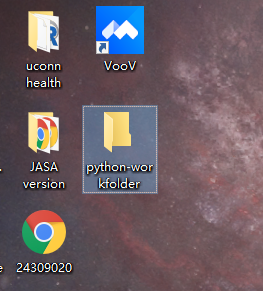
\includegraphics[width=4cm]{images/fig6.png}}
	\end{picture}
}

\uncover<2->
{
	\begin{picture}(0,0)(0,0)
		\put(90,-120)
		{
\includegraphics[width=4cm]{images/fig7.png}}
	\end{picture}
}
\end{frame}

\begin{frame}[fragile]{Folder tree in jupyter notebook}
\uncover<1->
{
	\begin{picture}(0,0)(0,0)
		\put(10,-80)
		{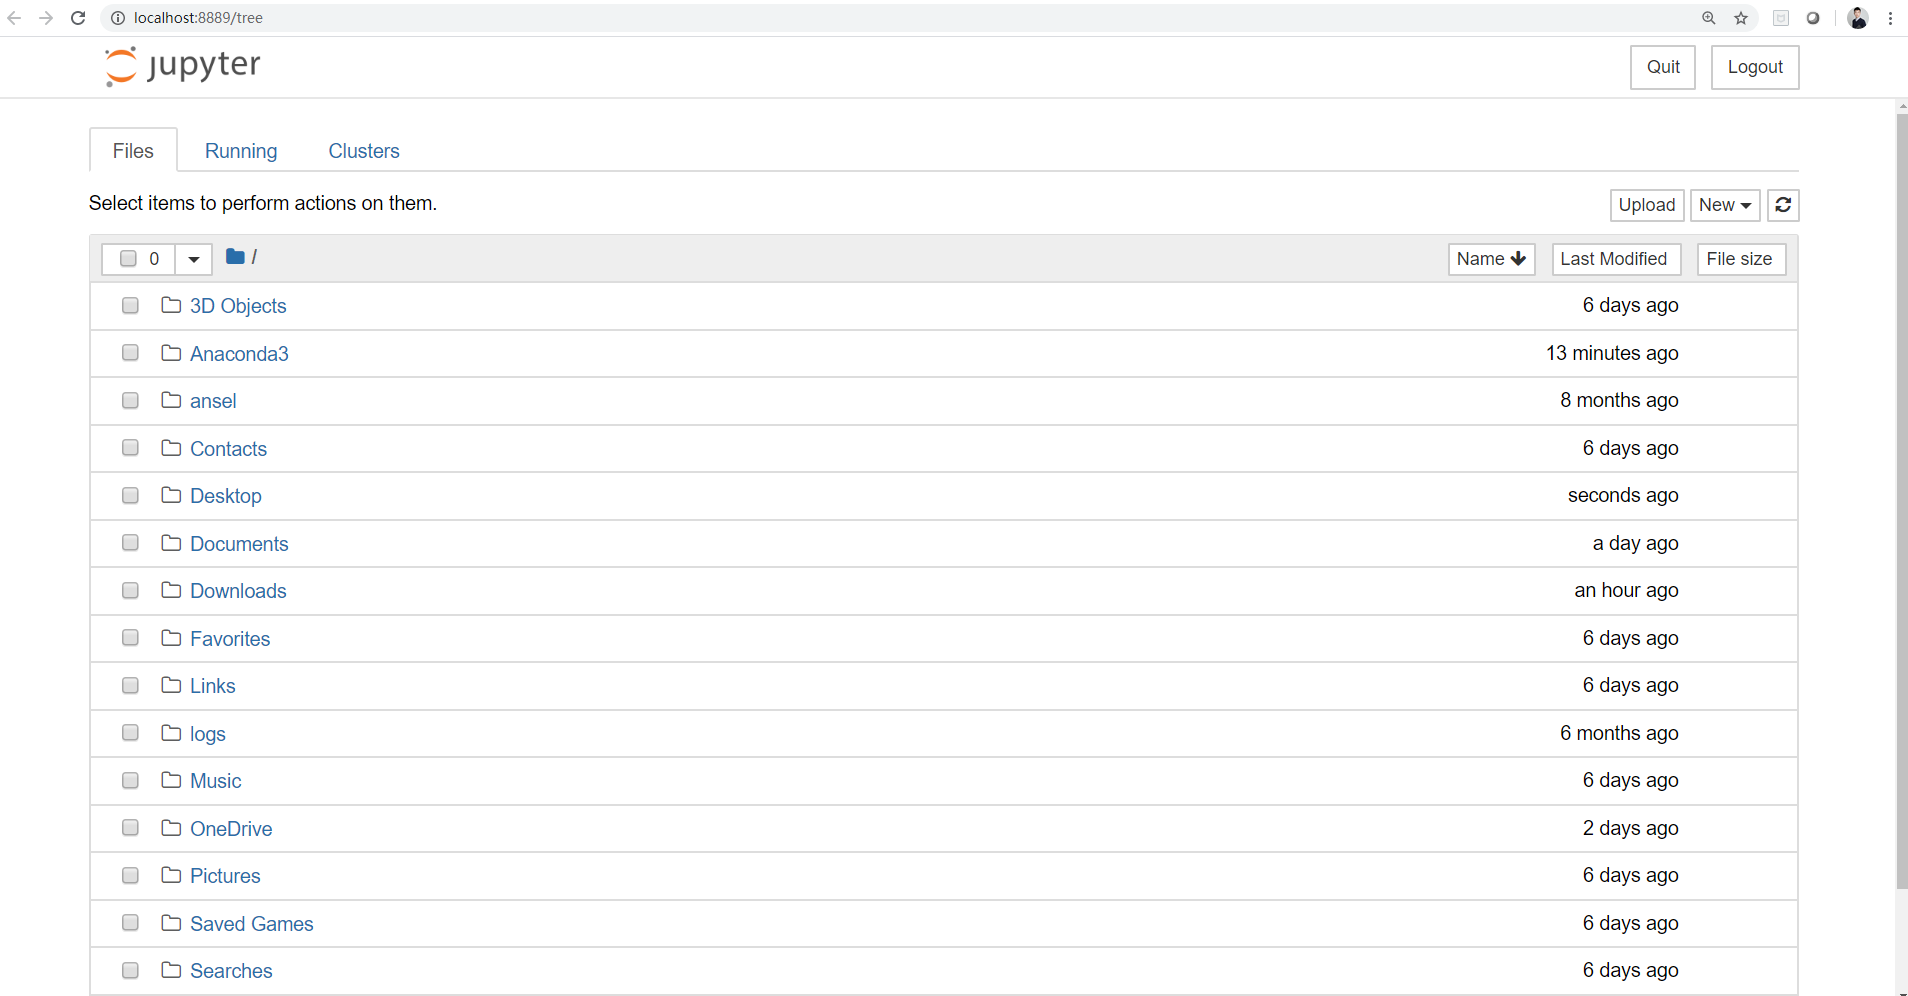
\includegraphics[width=9cm]{images/fig8.png}}
	\end{picture}
}

\uncover<2->
{
	\begin{picture}(0,0)(0,0)
		\put(90,-120)
		{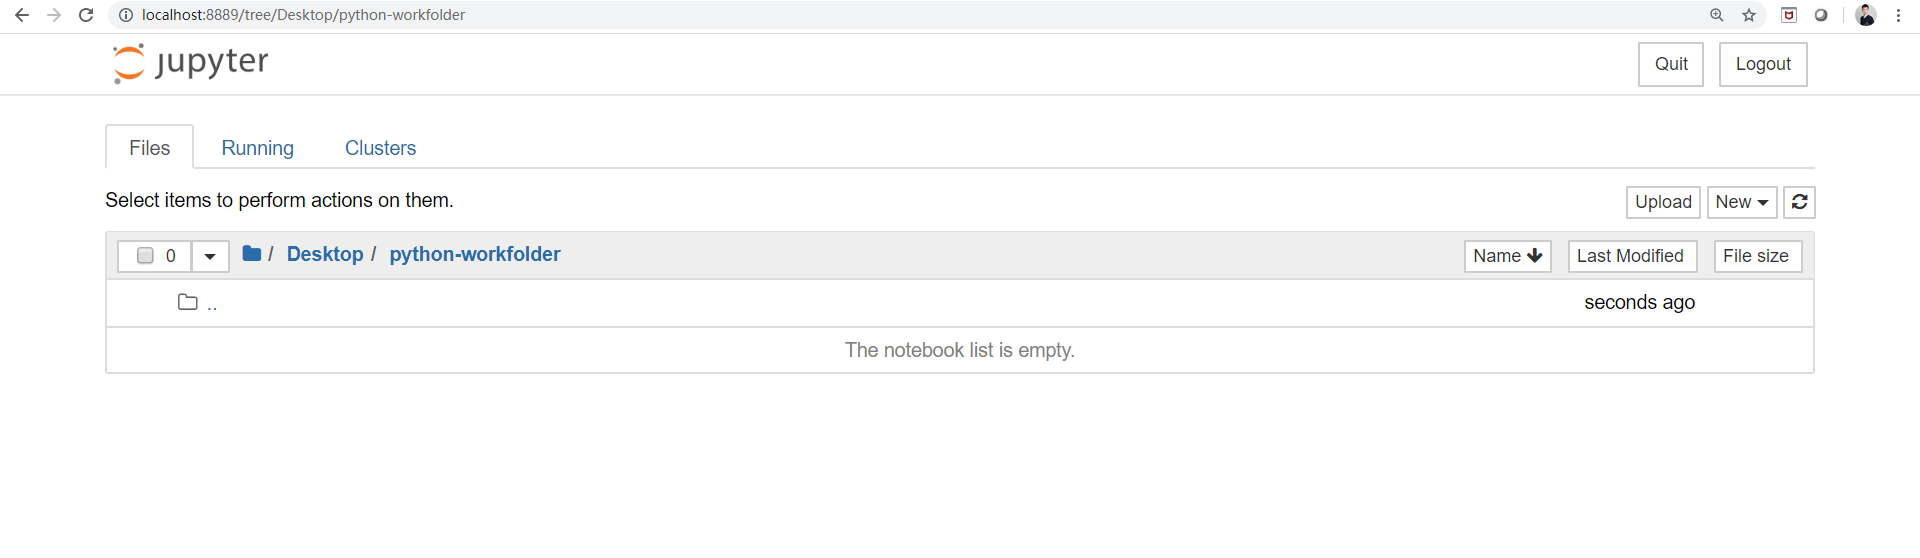
\includegraphics[width=9cm]{images/fig9.png}}
	\end{picture}
}
\end{frame}

\begin{frame}[fragile]{Create the first python script}
\uncover<1->
{
	\begin{picture}(0,0)(0,0)
		\put(10,-30)
		{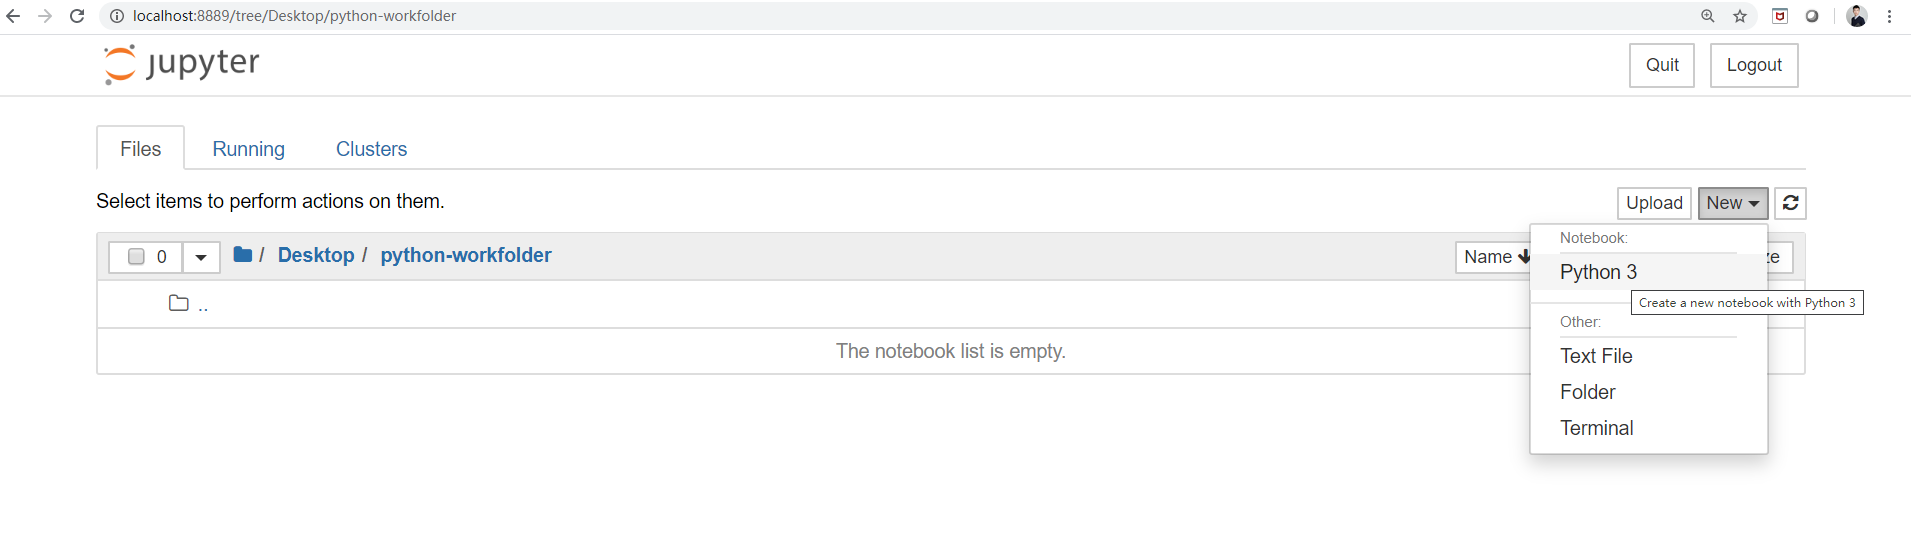
\includegraphics[width=10cm]{images/fig10.png}}
	\end{picture}
}

\uncover<2->
{
	\begin{picture}(0,0)(0,0)
		\put(10,-70)
		{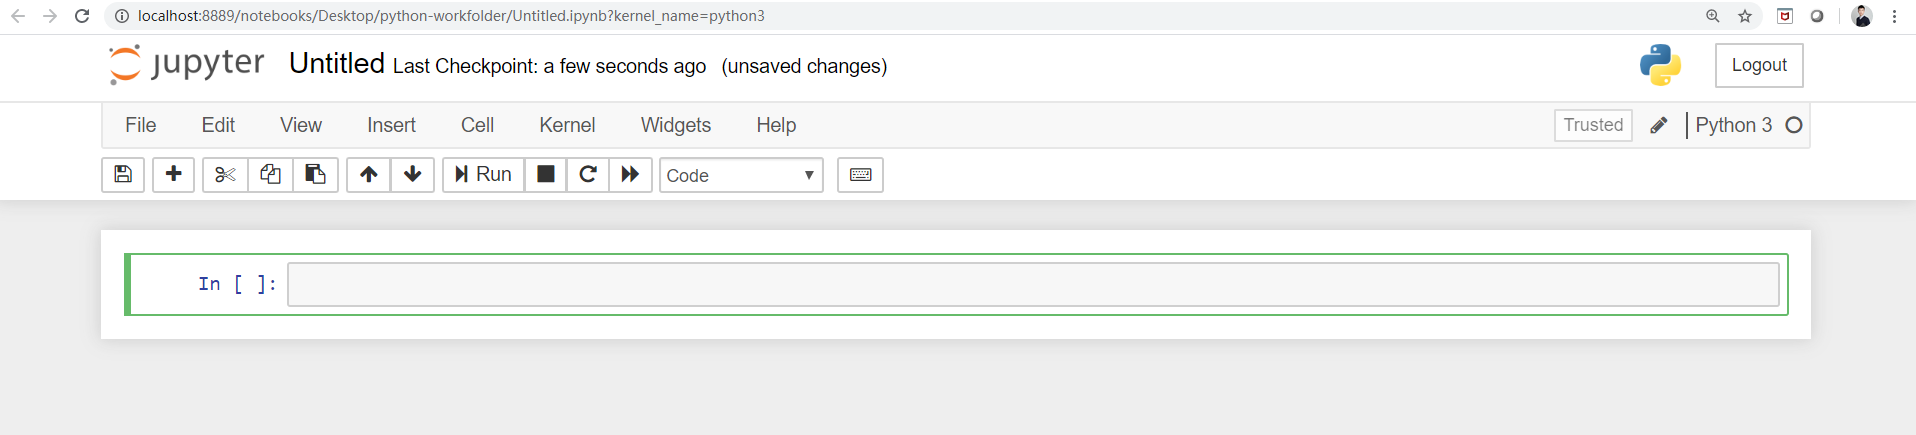
\includegraphics[width=10cm]{images/fig11.png}}
	\end{picture}
}
\end{frame}

\begin{frame}{Useful info}

The material of this session is in \href{https://github.com/brucejunjin/ucsas2020-introduction-to-python}{\tt \textcolor{blue}{Session Material}}.
\par
Our department website is \href{https://stat.uconn.edu/}{\tt \textcolor{blue}{Department of Statistics}}.
\par
Our website for statistical data science lab at Uconn is \href{https://statds.org/}{\tt \textcolor{blue}{Data Science Lab}}.

\end{frame}

\end{document}

